\documentclass{standalone}
\usepackage{tikz}
\usetikzlibrary{calc, shapes, backgrounds}
\usepackage{standalone}
\usepackage{amsmath, amssymb}
\begin{document}

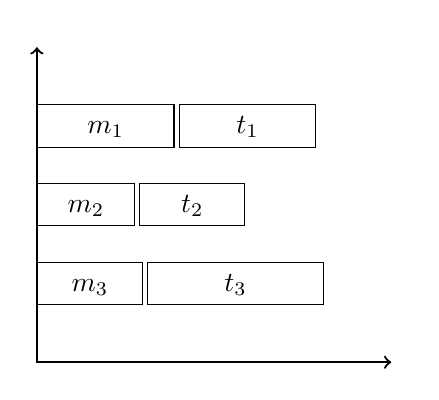
\begin{tikzpicture}
\tikzset{VertexStyle/.style = {anchor= west, draw, align= center, text height= 2.5mm}
}

    % Draw axes
    \draw [<->,thick] (0,4) node (yaxis) [above] {}
        |- (45mm,0) node (xaxis) [right] {};

   \node[VertexStyle, text width= 15mm] (rect1) at (0mm,3)  {$m_1$};
   \node[VertexStyle, text width= 15mm] (rect2) at (18mm,3) {$t_1$};
   
   \node[VertexStyle, text width= 10mm] (rect1) at (0mm,2)  {$m_2$};
   \node[VertexStyle, text width= 11mm] (rect2) at (13mm,2) {$t_2$};
      
   \node[VertexStyle, text width= 11mm] (rect1) at (0mm,1)  {$m_3$};
   \node[VertexStyle, text width= 20mm] (rect2) at (14mm,1) {$t_3$};
\end{tikzpicture}
\end{document} 
